\documentclass[a4paper, 11pt, oneside]{book}
\usepackage[a4paper, total={6.5in, 10in}]{geometry}
\usepackage{hyperref}

\usepackage[svgnames]{xcolor}
\usepackage{graphicx}
\usepackage[utf8]{inputenc}
\usepackage[T1]{fontenc}
\usepackage{PTSerif}
\usepackage{listings}
\usepackage{booktabs}
\usepackage{fouriernc}
\usepackage{makecell}
\usepackage{fontawesome}
\usepackage{hyperref}
\usepackage{tabularx}
\usepackage{xparse}
\usepackage[many]{tcolorbox}
\tcbuselibrary{listings}


\begin{document}



\begin{titlepage}
    \thispagestyle{empty}
    \centering
    
\includegraphics[scale=.4]{graphics/cx_logo-dark.png}
    \vfill
    \textcolor{Sienna}{\Huge CxAnalytix 2.x}
    \vfill
    {\Large\textbf{Nathan Leach, CSSLP\\Checkmarx Principal Solution Architect}}
\end{titlepage}

\newpage


\tableofcontents

\chapter*{Foreward}

As vulnerability scans are performed, a significant amount of data is generated over time.  The
scan data is normally consumed by development teams to remediate issues found in their specific 
projects.  The development team will perform triage and code changes as they assess what is required 
from the scan results. 

CxAnalytix was created when managment teams expressed the desire to create dashboards with
aggregated views of vulnerabilities across all scanning activity.  While CxAnalytix itself
does not produce these dashboards, it crawls scan results and collects the vulnerability
data that is then integrated into custom dashboards.\\\\

CxAnalytix currently supports the following Checkmarx products:

\begin{itemize}
    \item Checkmarx SAST (including OSA and Management \& Orchestration)
    \item Checkmarx SCA
\end{itemize}

The documentation for CxAnalytix was moved from the GitHub Wiki as of version 2.0.  This
manual will serve as the source of CxAnalytix documentation.  The manual will be updated
and versioned with each CxAnalytix release.

\newtcblisting{xml}[3]{
    listing only,
    title=<#1> #2 #3,
    width=\textwidth,
    listing options={
        basicstyle=\small\ttfamily,
        breaklines=true,
        columns=fullflexible,
    },
}

\newtcblisting{code}[3]{
    listing only,
    title=#1 #2 #3,
    width=\textwidth,
    listing options={
        basicstyle=\small\ttfamily,
        breaklines=true,
        columns=fullflexible,
    },
}


\part{Operation}
\chapter{Quickstart}

CxAnalytix performs read-only operations using Checkmarx REST APIs to obtain vulnerability data. It is therefore possible to execute 
CxAnalytix locally (e.g. on your workstation\footnote{Depending on the number of scans that need to be crawled, you may need a significant amount of disk space.}) 
or on a test system without the need to make any production changes.\\

\noindent The requirements to execute a test crawl are:

\begin{enumerate}
    \item Download the \href{https://github.com/checkmarx-ts/CxAnalytix/releases}{latest release zip}
    \item Unzip the release binaries into a directory of your choice
    \item Update the configuration with:
    \begin{itemize}
        \item The URL of the REST API endpoint(s)
        \item Credentials to access the REST API endpoint(s)
    \end{itemize}    
\end{enumerate}


\section{Quick SAST Crawl}


Some basic configuration is required before execution.

\begin{enumerate}
    \item Open a command prompt.
    \item Switch to the directory containing the CxAnalytix binaries.
    \item Set the environment variable \verb|CHECKMARX_URL| to the URL of your SAST instance.\footnote{Do not include "cxwebclient" in your SAST URL!}
    \item Set the environment variable \verb|CHECKMARX_USERNAME| to a SAST application user account name.
    \item Set the environment variable \verb|CHECKMARX_PASSWORD| to the password for the SAST application user account.
    \item Set the environment variable \verb|CHECKMARX_STATE_PATH| to a path where the state data will be stored.  
    A path of \verb|.| or any other temporary storage location is sufficient for evaluation.
    \item Execute \verb|CxAnalytixCLI| (Linux) or \verb|CxAnalytixCLI.exe| (Windows)
\end{enumerate}

The SAST vulnerability data will be retrieved and written to files in the \verb|logs| directory located in the directory where the CxAnalytix binaries
have been extracted.  If the crawl is interrupted, it will be re-started from the scan being processed when the crawl was interrupted.  To completely 
re-start the crawl, find and delete the \verb|CxAnalytixExportState.json| file in the directory specified by the \verb|CHECKMARX_STATE_PATH| 
environment variable.

\chapter{Deployment Guide}


\section{Hardware Requirements}

CxAnalytix is recommended to run on a standalone server or as a Docker container. It can run on the CxSAST manager 
as it does not tend to have an extremely CPU intensive workload for most scan volumes. It is not recommended to run it on the CxSAST manager 
if it can be avoided.

\noindent\\
Basic runtime specification:
    \begin{itemize}
        \item 4GB RAM
        \item CPU Cores should be 1 more than the configured number of concurrent scan threads (i.e. \textit{number of threads} + 1)
        \item At least 1TB of space if storing extraction data for 2 weeks or less if you expect < 100 scans every 2 hours
    \end{itemize}

\noindent\\CxAnalytix can run on any version of Linux or Windows that supports .Net 6.0.  The CxAnalytix distribution is built
as a standalone executable; this means that it is not required to install .Net 6.0 on the platform.  For some Linux distributions,
additional packages may need to be installed that are dependencies of .Net 6.0 before CxAnalytix will execute.

\section{MongoDB Sizing}

The MongoDB instance can be one of the following types of MongoDB:

\begin{itemize}
    \item Native MongoDB (local or cloud)
    \item AWS DocumentDB
\end{itemize}

\noindent Other types of MongoDB API compatible document databases may also work.  Azure's CosmoDB is currently not recommended at this time due to the 
maximum 2MB document size.  When CosmoDB officially supports the 16MB document size, it may be a viable option.

\noindent\\If persisting the extracted data in MongoDB, there is no set guide to sizing. Several variables should be considered in selection of system sizing.

\begin{itemize}
    \item Data Retention\\
    Most deployments intend to persist the vulnerability data in perpetuity (or don't have a plan to purge data). 
    If this is the case, a MongoDB cluster with the ability to expand storage should be considered. This storage expansion will likely need to consider 
    sharding configurations that can be done as part of the MongoDB server configuration or via embedding a shard key directly in the stored data. 
    The \nameref{ShardKeyCookbook} can assist with choosing an appropriate configuration.

    \item Shard Searching\\
    Most searches for vulnerability data may not be done such that a specific set of shards can limit the scope of where the query is executed. This may result
    in searches across all shards. The expected volume of queries that may result in multi-shard searches should be taken into account when specifying the 
    cluster members' hardware specifics. The machine specification will also need to account for CPU required for any indexing and data ingestion.
\end{itemize}

\section{Network Connectivity Requirements}

\subsection{SAST Connections Diagram}
Figure \ref{fig:SAST-network} shows the connection diagram for a CxAnalytix deployment. Where connections to REST APIs are indicated, the transport mechanism is 
HTTP/s over any port specified by the URL. Where connections to the SQL database are indicated, the connection is a regular socket using SQL server's wire protocol.

\noindent\\It is not recommended that the SQL server connection be exposed to the public internet. The SQL connection exists to support the audit log export capability 
and is not required to run CxAnalytix.\footnote{SQL connectivity is not available for Checkmarx hosted environments.}

\begin{figure}[h]
    \caption{SAST Network Connection Diagram}
    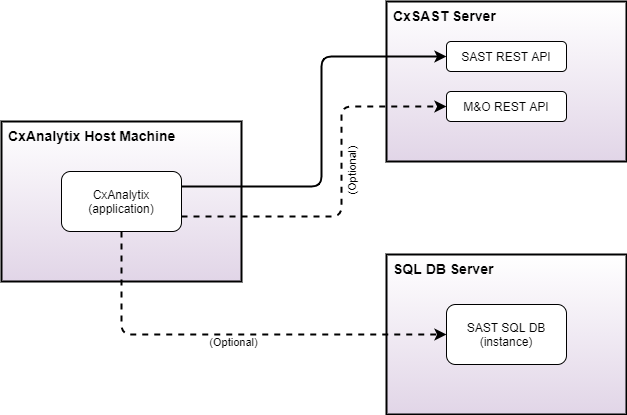
\includegraphics[width=\textwidth]{graphics/Deployment-SAST-connections.png}
    \label{fig:SAST-network}
\end{figure}

\subsection{Splunk Deployment Diagram}
Figure \ref{fig:SPLUNK-network} shows a typical deployment of CxAnalytix with the Splunk Universal Forwarder. In this deployment,
the Universal Forwarder is configured to read the CxAnalytix log output and forward the data to a remote Splunk instance. The vulnerability 
data log locations are configured in the Log4Net configuration.

\noindent\\The Splunk Universal Forwarder should be configured to tail the CxAnalytix output, which will forward to Splunk.

\begin{figure}[h]
    \caption{Splunk Network Connection Diagram}
    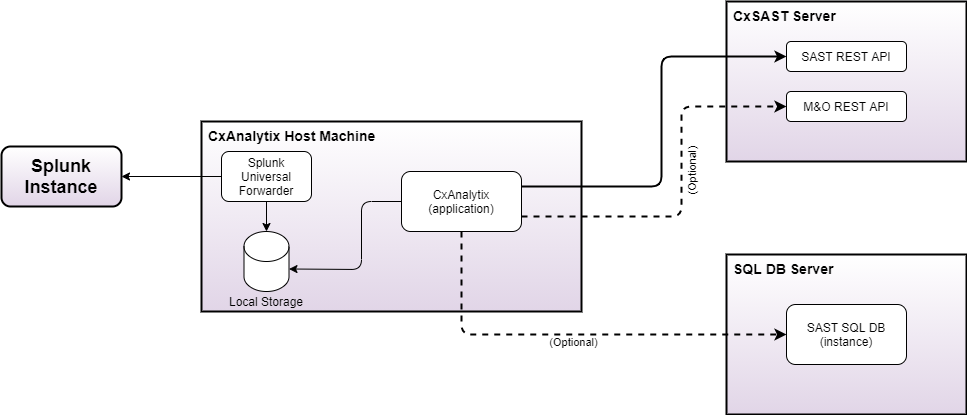
\includegraphics[width=\textwidth]{graphics/Deployment-SPLUNK-connections.png}
    \label{fig:SPLUNK-network}
\end{figure}


\subsection{MongoDB Deployment Diagram}
Figure \ref{fig:MONGO-network} shows a typical deployment of CxAnalytix configured to write vulnerability data to a MongoDB database. 
The MongoDB instance may be an on-premise instance or an instance hosted in the cloud.

\begin{figure}[h]
    \caption{MongoDB Network Connection Diagram}
    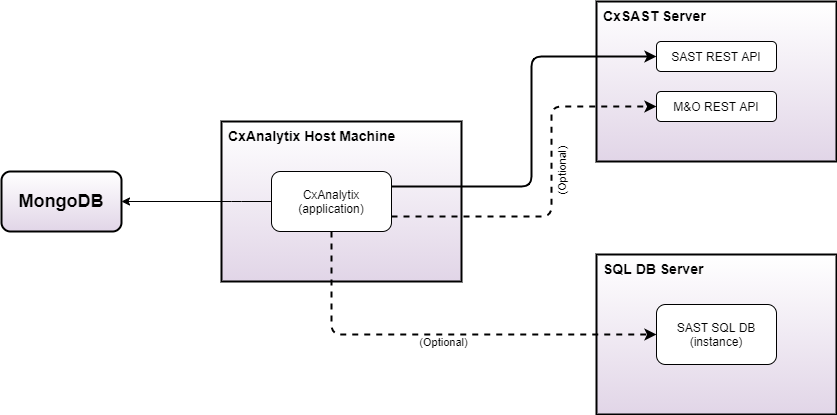
\includegraphics[width=\textwidth]{graphics/Deployment-MONGO-connections.png}
    \label{fig:MONGO-network}
\end{figure}


\section{Configuration Backups}
The crawl state storage files should be archived periodically to ensure crawling does not re-crawl existing scans. The state files are written to the path 
specified by the \verb|StateDataStoragePath| attribute in the \verb|CxAnalytixService| configuration section.  All files written to this path should
be archived periodically.

\noindent\\If running CxAnalytix as a Docker container, the default location \verb|/var/cxanalytix| should be mapped to a volume so that the state files are persistent across 
Docker container executions.  

\noindent\\The \verb|cxanalytix.config| file may also contain configurations that would be difficult to recreate.  It is advised that the configuration file be archived
after each change.

\section{Application Service Account}

An application service account is required for each service that CxAnalytix is configured to crawl.  If there are log messages indicating 
\verb|403: Forbidden| service API methods, this usually indicates the CxAnalytix role does not have appropriate privileges for that service.


\subsection{SAST}
CxAnalytix requires a SAST service account to authenticate with the SAST APIs to crawl scans. The service account has the following requirements:

\begin{itemize}
    \item The service account should be assigned at a team level that allows visibility to all projects that require crawling. 
    Usually this is the \verb|/CxServer|
    team but will depend on your configured team heirarchy. Any projects assigned to teams above or at a sibling level of the service account's assigned team 
    will not be visible to crawling requests.

    \item A role named CxAnalytix should be created and assigned to the service account user. The role should have the following minimum permissions:
    \begin{itemize}
        \item SAST->Project \& Scans->Save Sast Scan
        \item Reports->Generate Scan Reports
    \end{itemize}

\end{itemize}

\subsection{SCA}

CxAnalytix requires an SCA service account authenticate with the SCA APIs to crawl scan reports. The service account has the following requirements:

\begin{itemize}
    \item The service account should be assigned at a team level that allows visibility to all projects that require crawling. 
    Usually this is the \verb|/CxServer|
    team but will depend on your configured team heirarchy. Any projects assigned to teams above or at a sibling level of the service account's assigned team 
    will not be visible to crawling requests.

    \item A role named CxAnalytix should be created and assigned to the service account user. The role should have the following minimum permissions:
    \begin{itemize}
        \item SCA Viewer
    \end{itemize}

\end{itemize}


\chapter{Installation}\label{chap:installation}

\newcommand{\configstmt}[2]{
\subsection{Configuration File Path Resolution}\label{plat:#1}
    
The \texttt{cxanalytix.config} and \texttt{cxanalytix.log4net} configuration files are included in the distribution zip by default.  These
files can be left in the same directory as the runtime or deployed to different paths to make upgrades easier to manage.\\

\noindent\\On the #1 platform, the search path is:\\
\begin{enumerate}
    \item The current working directory of the running application.
    \item The path specified by the \texttt{CXANALYTIX\_CONFIG\_PATH} environment variable.
    \item The directory path \texttt{#2}.
\end{enumerate}
}

\newcommand{\clistmt}[2]{
    \subsection{CxAnalytix CLI}
    The CxAnalytix CLI provides a method of invoking a one-time crawl.  It is recommended that any crawling services running in the background
    are stopped before invoking the CLI.

    \noindent\\On the #1 platform, the \texttt{CxAnalytixCLI#2} executable can be run from any path.  The CLI follows the search logic described in section \ref{plat:#1}.
}


\section{Installing on Windows}
\newcommand{\windowsconfigpathbase}{\%PROGRAMDATA\%/cxanalytix}
\newcommand{\windowsconfigpath}{\windowsconfigpathbase/cxanalytix.config}
\configstmt{Windows}{\windowsconfigpath}
\clistmt{Windows}{.exe}

\subsection{CxAnalytix Service}
\begin{enumerate}
    \item Open Powershell or Windows command prompt as administrator.
    \item Execute: \texttt{sc.exe create CxAnalytix binpath="\{install folder path\}/CxAnalytixService.exe"}
    \item Make the directory \texttt{\windowsconfigpathbase}
    \item Move the \texttt{cxanalytix.config} and \texttt{cxanalytix.log4net} \\to \windowsconfigpathbase.
    \item Ensure permissions for the folder \texttt{\windowsconfigpathbase} allow Read/Write access to the service account that is running
    CxAnalytixService.\footnote{Usually this is set to SYSTEM by default and does not need modification.}
\end{enumerate}



\noindent\\The CxAnalytix service and now be started and stopped from the Service Control Manager.


\section{Installing on Linux}
\configstmt{Linux}{/etc/cxanalytix}
\clistmt{Linux}{}

\subsection{CxAnalytix Daemon}
There is not a platform-specific installer for CxAnalytix at the time this documentation was written. The following steps can 
be used to install the CxAnalytix Daemon on a Linux system that uses \verb|systemd|\footnote{Perform the installation steps as the root user.}.


\begin{enumerate}
    \item Configure the system running CxAnalytix to have the same time zone as the SAST Manager if SAST scans will be crawled.
    \footnote{SAST uses localtime for some time fields; this may make some scans to be 
    crawled with a delay equal to the time zone difference between CxAnalytix and the SAST Manager.}

    \item Make directory \texttt{/var/log/cxanalytix}

    \item Execute \texttt{chown root:nobody /var/log/cxanalytix}

    \item Execute \texttt{chmod g+w /var/log/cxanalytix}

    \item Make directory \texttt{/etc/cxanalytix}

    \item Move the \texttt{cxanalytix.config} and \texttt{cxanalytix.log4net} files to \texttt{/etc/cxanalytix}

    \item Execute: \texttt{chown root:nobody /etc/cxanalytix}

    \item Execute \texttt{chmod g+w /etc/cxanalytix}

    \item Make the directory \texttt{/opt/cxanalytix} and copy the installation artifacts there.

    \item Execute: \texttt{chown root:nobody /opt/cxanalytix}

    \item Modify the \texttt{cxanalytix.log4net} file to output logs into \texttt{/var/log/cxanalytix}
    
    \item Copy the file \texttt{cxanalytix.service} to \texttt{/etc/systemd/system/}

    \item Enable automatic startup of the daemon by executing: \texttt{systemctl enable cxanalytix}

    \item \textit{(optional)} Start the daemon by executing: \texttt{systemctl start cxanalytix}

\end{enumerate}

\noindent\\After CxAnalytix is installed, modify the \texttt{cxanalytix.config} and/or \texttt{cxanalytix.log4net} files according to the 
configuration instructions in Chapter \ref{chap:configuration}.

\section{Running CxAnalytix as a Docker Container}

CxAnalytix is published as a docker image in the \href{https://github.com/checkmarx-ts/CxAnalytix/pkgs/container/cxanalytix%2Fcxanalytix}{Checkmarx TS} GitHub 
packages repository. You can reference the image using \verb|ghcr.io/checkmarx-ts/cxanalytix/cxanalytix:<tag>| where \verb|tag| can be:

\begin{itemize}
    \item \verb|latest| to get the latest release
    \item \verb|vx.x.x| to get a specific release version
    \item \verb|vx.x.x-x-prerelease| to get a specific build of a pre-release version
\end{itemize}

\subsection{Configuration with Environment Variables}

Several of the configuration fields support environment variable expansion.  The default configuration file will use the log4net output
module to place the data files in \verb|/var/logs/cxanalytix| table \ref{tab:env} shows the environment variables required for a 
basic CxAnalytix runtime configuration.

\begin{table}
    \centering
    \begin{tabular}{|c|c|l|}
        \toprule
        \textbf{Environment Variable} & \textbf{Default} & \textbf{Description}\\
        \midrule
        \verb|CHECKMARX_URL| & None & The URL to the SAST server.\\
        \midrule
        \verb|CHECKMARX_USERNAME| & None & The username of the account that will log into CxSAST.\\
        \midrule
        \verb|CHECKMARX_PASSWORD| & None & The password for the user account logging into CxSAST.\\
        \midrule
        \verb|CHECKMARX_STATE_PATH| & \verb|/var/cxanalytix| & The path where state files will be stored.\\
        \bottomrule
    \end{tabular}
    \caption{Docker configuration environment variables}
    \label{tab:env}
\end{table}

\noindent\\By default, the state storage path is \verb|/var/cxanalytix|. The state storage files will be lost after the Docker image exits unless a volume is mapped 
to \verb|/var/cxanalytix|. A custom configuration can be used to change the location of the state storage, or a volume can be mapped to 
\verb|/var/cxanalytix| to allow the state storage files to be persisted across container executions.


\subsection{Other Container Configuration Options}

Some of the configuration options in CxAnalytix can be too complex for using environment variables alone.  There are a few different options
that will allow for a user-supplied configuration to be used by the running container.

\subsubsection{Extending the CxAnalytix Docker Image}

The base docker image can be customized using \verb|FROM ghcr.io/checkmarx-ts/cxanalytix/cxanalytix:<tag>| and copying 
the \verb|cxanalytix.log4net| and \verb|cxanalytix.config| files to /etc/cxanalytix. You can refer to the Dockerfile to re-use the \verb|ENTRYPOINT| or 
provide your own entry point.

\noindent\\The state file storage location can be configured in the custom configuration files to write the state files at a location where a 
volume is mapped.  This will allow the state to persist across container executions.


\subsubsection{Volume Mapping}

Volume or host path mounts can be mounted to various locations when running the CxAnalytix Docker image.  Table \ref{tab:mounts} shows
the paths that should be considered for volume mounting.

\begin{table}
    \centering
    \begin{tabular}{|l|l|}
        \toprule
        \textbf{Location} & \textbf{Description}\\
        \midrule
        \verb|/etc/cxanalytix| & \makecell[l]{Place the \texttt{cxanalytix.log4net} and \texttt{cxanalytix.config} configuration files here.
        \\The daemon will run and use these files to configure the runtime.}\\
        \midrule
        \verb|/var/cxanalytix| & This is where the state files are written as scans are crawled.\\
        \midrule
        \verb|/var/logs/cxanalytix| & If configured to output to log files, this is where the log files are written by default.\\
        \bottomrule
    \end{tabular}
    \caption{Container Mount Locations}
    \label{tab:mounts}
\end{table}


\section{Logging Configuration}

Log4Net is used to produce both application logs and logs containing exported JSON key/value pairs when using the Logging Output component. 
CxAnalytix produces logging useful for troubleshooting and/or execution tracking purposes even when not using the Log4Net output method.  The 
\texttt{cxanalytix.log4net} file is generally located in the same directory as the \texttt{cxanalytix.config} file, and will allow for
customizing the logging output location and verbosity.



\section{Upgrading}


Configuration elements found in \texttt{cxanalytix.config} are generally backwards compatible for versions
of CxAnalytix with the same major version\footnote{The major version is the first 
number in the version stamp.  e.g. v2.0.0 has a major version of 2.}.  New features may require additions
to the \texttt{cxanalytix.config} file. Please refer to Chapter \ref{chap:configuration} for additional details
about modifying the configuration file.


\noindent\\When configuring CxAnalytix, it is recommended that the configuration, state, and log files are stored
in directories separate from the CxAnalytix binaries.  This will prevent the inadvertent misconfiguration on upgrade.


\noindent\\Note that if installing from the CxAnalytix zip binary that there is a default version of \texttt{cxanalytix.config}
and \texttt{cxanalytix.log4net} in the zip binary.  These default configuration files can safely be removed upon
upgrading the CxAnalytix binaries.

\chapter{Configuration}\label{chap:configuration}


\newcommand{\configelement}[2]{\paragraph{XML Element: #1, Expands: #2}}

CxAnalytix uses the XML \texttt{cxanalytix.config} to configure the application execution parameters.  A path search order described in chapter \ref{chap:installation}
describes how CxAnalytix finds the configuration file at runtime.

\noindent\\Configuration of CxAnalytix is performed by adding XML elements to the top level \texttt{configuration} element in the
\texttt{cxanalytix.config} file.  The XML element names are indicated in each section with an example set of XML attributes or child-elements.

\noindent\\Elements that are noted as "Expands" will expand environment variables for assigned to elements for environment variable values in the
format \texttt{\%VARIABLENAME\%}.  

\section{General Configuration}\label{sec:general}

\subsection{Never Do This}

The \texttt{cxanalytix.config} file needs to be modified to supply the appropriate configuration elements.  The \texttt{configSections}
element is not intended to be user configurable.  Listing \ref{lst:motouch} shows an example of the contents of this XML element;
\textbf{never change anything in this section.}

\begin{lstlisting}[caption={Part of the Configuration File to Never Change}, label={lst:motouch}, language=XML, basicstyle=\ttfamily\tiny]
<configSections>
    <section name="CxAnalytixService" 
        type="CxAnalytix.Configuration.Impls.CxAnalytixService, Configuration" />
    <section name="CxSASTCredentials" 
        type="CxAnalytix.Configuration.Impls.CxCredentials, Configuration" />
    <section name="CxSCACredentials" 
        type="CxAnalytix.Configuration.Impls.CxMultiTenantCredentials, Configuration" />
    <section name="CxSASTConnection" 
        type="CxAnalytix.Configuration.Impls.CxSASTConnection, Configuration" />
    <section name="CxSCAConnection" 
        type="CxAnalytix.XForm.ScaTransformer.Config.CxScaConnection, ScaTransformer" />
    <section name="ProjectFilterRegex" 
        type="CxAnalytix.Configuration.Impls.CxFilter, Configuration"/>
    <section name="CxAuditTrailSuppressions" 
        type="CxAnalytix.AuditTrails.Crawler.Config.CxAuditTrailSuppressions, CxAuditTrailsCrawler"/>
    <section name="CxAuditTrailRecords" 
        type="CxAnalytix.AuditTrails.Crawler.Config.CxAuditTrailRecordNameMap, CxAuditTrailsCrawler"/>
    <section name="CxDB" 
        type="CxAnalytix.CxAuditTrails.DB.Config.CxAuditDBConnection, CxAuditTrailsDB"/>
    <section name="AMQPConnection" 
        type="CxAnalytix.Out.AMQPOutput.Config.Impls.AmqpConnectionConfig, AMQPOutput"/>
    <section name="AMQPConfig" 
        type="CxAnalytix.Out.AMQPOutput.Config.Impls.AmqpConfig, AMQPOutput"/>
    <section name="CxLogOutput" 
        type="CxAnalytix.Out.Log4NetOutput.Config.Impl.LogOutputConfig, Log4NetOutput" />
    <section name="CxMongoOutput" 
        type="CxAnalytix.Out.MongoDBOutput.Config.Impl.MongoOutConfig, MongoDBOutput" />
    <section name="CxMongoConnection" 
        type="CxAnalytix.Out.MongoDBOutput.Config.Impl.MongoConnectionConfig, MongoDBOutput" />
</configSections>
\end{lstlisting}


\subsection{Checkmarx Service Connection Configuration}

\subsubsection{Checkmarx SAST Connection Configuration}

\configelement{CxSASTConnection}{Yes}

\noindent\\\\\textbf{Expands Environment Variables}

\noindent\\Example:

\noindent\\\texttt{
CxSASTConnection\\\indent URL=""
\\\indent mnoURL=""
\\\indent TimeoutSeconds="" 
\\\indent ValidateCertificates="true"
\\\indent RetryLoop=""
\\\indent />
}\\\\

\begin{table}[h]
    \caption{CxSASTConnection Attributes}        
    \begin{tabular}{|c|c|c|l|}
        \toprule
        \textbf{Attribute} & \textbf{Default} & \textbf{Required} & \textbf{Description}\\
        \midrule
        \texttt{URL} & N/A & Yes & \makecell[l]{The URL to the SAST server.}\\
        \midrule
        \texttt{mnoURL} & N/A & No & \makecell[l]{The URL to the Management and Orchestration endpoint\\of the SAST server.}\\
        \midrule
        \texttt{TimeoutSeconds} & 300 & No & \makecell[l]{The number of seconds to wait until an\\API operation times out.}\\
        \midrule
        \texttt{ValidateCertificates} & True & No & \makecell[l]{Validate SSL certificates for\\API endpoints.}\\
        \midrule
        \texttt{RetryLoop} & 0 & No & \makecell[l]{The number of retries for an API operation\\after the operation times out.}\\
        \bottomrule
    \end{tabular}
\end{table}


\subsubsection{Checkmarx SCA Connection Configuration}


\subsection{CxAnalytix Service and CLI Execution Configuration}


\section{Splunk Output Configuration}\label{sec:splunk_config}
\subsection{Log4Net Output Configuration}

The Log4Net output is used to generate log files that are tailed and forwarded to Splunk via the Splunk Universal Forwarder.  This requires the Log4Net
output to be configured so that the Universal Forwarder can find the generated output files.

\noindent\\The Log4Net configuration file should be modified only to change the output path of the generated data output files.  The generated data output files are different
than the application logging output files in that the data output files contain data to be used for analysis purposes. It may be desirable to also forward
the application log files to Splunk for monitoring and troubleshooting purposes.

\noindent\\The \texttt{CxAnalytixService} configuration section in \texttt{cxanalytix.config} contains record name mapping attributes.  Listing \ref{lst:record_map}
shows an example configuration with the record names mapped to file logger names shown configured in listing \ref{lst:record_loggers}.  The loggers
reference file appenders, as seen in listing \ref{lst:record_appenders}.  The appender configuration, by default, places all output in the \texttt{logs}
directory, which resolves to the current working directory set when a CxAnalytix process executes.  The location of the output files can be changed
by modifying the appender configuration in \texttt{cxanalytix.log4net}.


\begin{lstlisting}[caption={Example Record Map Configuration}, label={lst:record_map}, language=XML]
<CxAnalytixService 
    ConcurrentThreads="2" 
    StateDataStoragePath="%CHECKMARX_STATE_PATH%"
    ProcessPeriodMinutes="120"
    OutputModuleName="log4net"
    SASTScanSummaryRecordName="RECORD_SAST_Scan_Summary"
    SASTScanDetailRecordName="RECORD_SAST_Scan_Detail"
    SCAScanSummaryRecordName="RECORD_SCA_Scan_Summary"
    SCAScanDetailRecordName="RECORD_SCA_Scan_Detail"
    ProjectInfoRecordName="RECORD_Project_Info"
    PolicyViolationsRecordName="RECORD_Policy_Violations">
    <EnabledTransformers>
        <Transformer Name="SAST" />
    </EnabledTransformers>
</CxAnalytixService>
\end{lstlisting}

\begin{lstlisting}[caption={Log4Net Logger Configurations}, label={lst:record_loggers}, language=XML]
.. snip ..
<logger name="RECORD_SAST_Scan_Summary" aditivity="false">
    <level value="ALL" />
    <appender-ref ref="SAST_SS" />
</logger>
  .. snip ..
\end{lstlisting}

\begin{lstlisting}[caption={Log4Net Record File Appenders}, label={lst:record_appenders}, language=XML]
.. snip ..
<appender name="SAST_SS" type="log4net.Appender.RollingFileAppender">
    <appendToFile value="true" />
    <maximumFileSize value="100MB" />
    <rollingStyle value="Composite" />
    <staticLogFileName value="false" />
    <countDirection value="1" />
    <file type="log4net.Util.PatternString" value="logs/sast_scan_summary" />
    <datePattern value="'.'yyyy_MM_dd'.log'" />
    <preserveLogFileNameExtension value="true" />

    <layout type="log4net.Layout.PatternLayout">
        <conversionPattern value="%message%newline" />
    </layout>
</appender>
.. snip ..
\end{lstlisting}

\subsection{Splunk Universal Forwarder Configuration}
The \ref{https://www.splunk.com/en_us/download/universal-forwarder.html}{Splunk Universal Forwarder} is used to send data to Splunk Enterprise or Splunk Cloud.  
Please refer to the Splunk website for information for details about installing and configuring the Universal Forwarder.


\subsubsection{Output File Tailing Configuration}

Assuming an installed forwarder is able to connect to the desired Splunk instance, 
create the \href{https://docs.splunk.com/Documentation/Splunk/latest/Admin/Inputsconf}{\texttt{inputs.conf}} file at the appropriate location 
(e.g. \texttt{/etc/apps/splunkclouduf/default/inputs.conf}).  Listing \ref{lst:inputsconf} shows an example of an \texttt{inputs.conf}
file with monitoring stanzas appropriate for each type of record. 

\begin{lstlisting}[caption={Log4Net Record File Appenders}, label={lst:inputsconf}, language=XML]
[monitor://{path to logs}\CxAnalytixService...]
sourcetype=service

[monitor://{path to logs}\sast_scan_summary...]
sourcetype=sast_scan_summary

[monitor://{path to logs}\sast_scan_detail...]
sourcetype=sast_scan_detail

[monitor://{path to logs}\sast_project_info...]
sourcetype=sast_project_info

[monitor://{path to logs}\sast_policy_violations...]
sourcetype=sast_policy_violation

[monitor://{path to logs}\sca_scan_summary...]
sourcetype=sca_scan_summary

[monitor://{path to logs}\sca_scan_detail...]
sourcetype=sca_scan_detail

[monitor://{path to logs}\CxActivity_dbo_AuditTrail...]
sourcetype=cxactivity_audittrail

[monitor://{path to logs}\CxActivity_dbo_Audit_Scans...]
sourcetype=cxactivity_auditscans

[monitor://{path to logs}\CxActivity_dbo_Audit_Reports...]
sourcetype=cxactivity_auditreports

[monitor://{path to logs}\CxActivity_dbo_Audit_Queries...]
sourcetype=cxactivity_auditqueries

[monitor://{path to logs}\CxActivity_dbo_Audit_Projects...]
sourcetype=cxactivity_auditprojects

[monitor://{path to logs}\CxActivity_dbo_Audit_Presets...]
sourcetype=cxactivity_auditpresets

[monitor://{path to logs}\CxActivity_dbo_Audit_DataRetention...]
sourcetype=cxactivity_auditdataretention
\end{lstlisting}

\subsubsection{Configuring the Source Types}

The source types on the Splunk server need to be configured to appropriately parse JSON.  
This can be done using \href{https://docs.splunk.com/Documentation/Splunk/latest/Admin/Propsconf}{\texttt{props.conf}} (only available in Splunk Enterprise) 
or through the Splunk UI. A source type should be created the matches each record output source types as defined in 
\href{https://docs.splunk.com/Documentation/Splunk/latest/Admin/Inputsconf}{\texttt{inputs.conf}}.  Listing \ref{lst:sourcetypes} shows an example
of a source type entry.  The source type configuration needs to be performed for each source type.


\begin{lstlisting}[caption={Log4Net Record File Appenders}, label={lst:sourcetypes}, language=XML]
LINE_BREAKER=([\r\n]+)
KV_MODE=json
TRUNCATE=0
SHOULD_LINEMERGE=false
\end{lstlisting}

\noindent\\\textbf{Extracting Timestamps}\\

\noindent\\The source data contains timestamp fields that can be used as the timestamp Splunk uses when indexing the data.  Without specifying how to extract the
timestamp from each source type, the timestamp will default to the timestamp when the data was indexed.  This may work for current data, but data searches 
will also return historical data that is outside of the selected search time frame.

\noindent\\For the SAST Scan Summary, SAST Scan Detail, SCA Scan Summary, and SCA Scan Detail source types, this configuration option should be added:

\noindent\\\texttt{TIME\_PREFIX=\^.*ScanFinished".+?"}

\noindent\\For the SAST Project Info source type, this configuration option should be added:

\noindent\\\texttt{TIME\_PREFIX=\^.*LastCrawlDate".+?"}

\noindent\\For the SAST Policy Violation source type, this configuration option should be added:

\noindent\\\texttt{TIME\_PREFIX=\^.*ViolationOccurredDate".+?"}

\noindent\\For the Audit Trail source type, this configuration option should be added:

\noindent\\\texttt{TIME\_PREFIX=\^.*EndTime".+?"}

\noindent\\For the Audit\_Scans, Audit\_Reports, Audit\_Queries, Audit\_Projects, Audit\_Presets, Audit\_DataRetention, this configuration option should be added:

\noindent\\\texttt{TIME\_PREFIX=\^.*TimeStamp".+?"}



\section{MongoDB Output Configuration}\label{sec:mongo_config}
\section{AMQP Output Configuration}\label{sec:amqp_config}

\section{Audit Table Crawling Configuration}


\section{Logging Configuration}

Log4Net is used to produce both application logs and logs containing exported JSON key/value pairs when using the Logging Output component. 
CxAnalytix produces logging useful for troubleshooting and/or execution tracking purposes even when not using the Log4Net output method.  The 
\texttt{cxanalytix.log4net} file is generally located in the same directory as the \texttt{cxanalytix.config} file, and will allow for
customizing the logging output location and verbosity.

\part{Development \& Data Analysis}
\chapter{Developing for CxAnalytix}

\section{Build From Source}

\subsection{The Easy Way}
The easiest method of building the code from source is to open the \texttt{CxAnalytix.sln} file using Visual Studio (not Visual Studio Code).
From there, the entire solution can be built with a "Build Solution" command.

\subsection{From the Command Line}
If the .Net Core SDK of the appropriate version is installed, the \texttt{dotnet} command can be executed to create a build:

\begin{lstlisting}
dotnet publish .\CxAnalytix.sln -o $OutLoc/win-x64 -c ReleaseWindows -r win-x64
dotnet publish .\CxAnalytix.sln -o $OutLoc/linux-x64 -c ReleaseLinux -r linux-x64
\end{lstlisting}

\subsection{Visual Studio Code}
This is a .Net Core application and therefore can be developed on any platform that supports .Net Core.  Readers are encouraged to investigate configuring
their instance of VSCode to build and debug CxAnalytix.  A basic \texttt{launch.json} and \texttt{tasks.json} file is included in the source tree, but they may need
updated as versions of .Net Core and VSCode change over time.


\section{Developing New Modules}

The transformation and output modules are dynamically loaded at runtime.  They are developed with an SDK component included in the CxAnalytix source tree.
The SDK component is intended to be used as a project reference at this time as it is not deployed as a Nuget package.

\noindent\\The modules, being that they are dynamically loaded, will have no incoming dependencies.  This means they will not be included
in the build output since the compiler will believe the shared libraries where the modules are implemented are not in use.  For easy debug and build
purposes, each output and transform module is added as a project dependency to the \texttt{Executive} project.  The \texttt{Executive} project
is loaded by executing applications on all platforms to perform the appropriate type of CxAnalytix execution.


\subsection{Creating New Transformation Modules}

Creating a new transformer type can be done with the following steps:

\begin{enumerate}
    \item Create a class library project.
    \item Add a project reference to \texttt{SDK.Modules}
    \item Create a class that derives from \texttt{TransformerModule}
    \item Create a public default constructor that initializes the transformer module with the runtime specifics of your module
    \item Implement the abstract methods/properties defined in \texttt{TransformerModule}
\end{enumerate}

\noindent\\An example transformer module can be observed in listing \ref{lst:xform}. The arguments passed to the \texttt{TransformerModule}
are explained in table \ref{tab:xform}.


\begin{table}
    \centering
    \begin{tabular}{|c|c|l|}
        \toprule
        \textbf{Argument} & \textbf{Type} & \textbf{Description}\\
        \midrule
        \texttt{moduleName} & \texttt{String} & \makecell[l]{The string used to select the module for invocation in the\\
        configuration as described in section \ref{sec:general} (e.g. SAST, SCA)}\\
        \midrule
        \texttt{moduleImplType} & \texttt{Type} & The .Net type that contains the implementation of the module.\\
        \midrule
        \texttt{stateStorageFileName} & \texttt{String} & The name of the file that stores any state of the transformation module.\\
        \bottomrule
    \end{tabular}
    \caption{\texttt{TransformerModule} Construction Parameters}
    \label{tab:xform}
\end{table}



\begin{lstlisting}[caption={Example Transformer Module}, label={lst:xform}, language=C]
class Transformer : TransformerModule
{
    public override string DisplayName 
        => "This is my module, this text will show in logs";

    
    public Transformer() 
        : base("MYMODULE", typeof(Transformer), "MYMODULE_state.json")
    {
        // Initialization goes here, if any
    }

    public override void DoTransform(CancellationToken token)
    {
        // This is where the transformation is executed.
    }
}
\end{lstlisting}

\subsection{Creating New Output Modules}

Output modules are created similarly to transformer modules.  The basic tasks to create an output module:

\begin{enumerate}
    \item Create a class library project.
    \item Add a project reference to \texttt{SDK.Modules}
    \item Create a class that derives from \texttt{OutputModule}; this is your factory class that creates the instance of the output implementation
    \item Create a public default constructor that initializes the output module with the runtime specifics of your module
    \item Implement the abstract methods/properties defined in \texttt{OutputModule}
\end{enumerate}

\noindent\\Listing \ref{lst:output} shows an example of an output implementation.  Table \ref{tab:output} explains the output
module arguments.


\begin{lstlisting}[caption={Example Output Module}, label={lst:output}, language=C]
public class MyOutFactory : SDK.Modules.Output.OutputModule
{
    public MyOutFactory() : base("MyOutput", typeof(MyOutFactory) )
    {
    }

    public override IRecordRef RegisterRecord(string recordName)
    {
        // Implementation for registering a record
    }

    public override IOutputTransaction StartTransaction()
    {
        // This is where the instance of the output implementation is given
        // to the caller.  Transactional capabilities are optional, the
        // concept of a transaction is simply a grouping of related
        // data being output.
    }
}    
\end{lstlisting}


\begin{table}
    \centering
    \begin{tabular}{|c|c|l|}
        \toprule
        \textbf{Argument} & \textbf{Type} & \textbf{Description}\\
        \midrule
        \texttt{moduleName} & \texttt{String} & \makecell[l]{The string used to select the module for output in the\\
        configuration as described in section \ref{sec:general} (e.g. MongoDB, AMQP, Log4Net)}\\
        \midrule
        \texttt{moduleImplType} & \texttt{Type} & The .Net type that contains the implementation of the module.\\
        \bottomrule
    \end{tabular}
    \caption{\texttt{OutputModule} Construction Parameters}
    \label{tab:output}
\end{table}


\section{Module Configuration}

\subsection{CxAnalytix Internal Configuration}\label{sec:internal_config}

It is possible to obtain the general configuration objects (described in section \ref{sec:general}) with a project dependency for the \texttt{Configuration}
class library.  Obtaining a reference to the \texttt{CxAnalytixService} configuration can then be achieved with the example code show in listing 
\ref{lst:global_config}.  Instances of CxAnalytix configuration objects can be obtained by specifying the type in the generic parameter for the 
method call \texttt{CxAnalytix.Configuration.Impls.Config.GetConfig<T>()} 

\begin{lstlisting}[caption={Retrieving a CxAnalytixService Config Object Instance}, label={lst:global_config}, language=C]
private CxAnalytixService Service => 
    CxAnalytix.Configuration.Impls.Config.GetConfig<CxAnalytixService>();
\end{lstlisting}


\subsection{Module-Specific Configuration}

All configurations in the \texttt{cxanalytix.config} file are consumed by the Microsoft\\ 
\texttt{System.Configuration.ConfigurationManager} package.
Each individual module implementation should define configuration classes that are publicly accessible for dynamic loading.
The assembly path for custom module configuration is then placed in the \texttt{configSections} element of the \texttt{cxanalytix.config}
file.  Listing \ref{lst:config_sections} shows an example of a configuration section entry to load the AMQP configuration elements
from the AMQP class library.

\noindent\\Obtaining an instance of a configuration object uses the same \texttt{GetConfig} as was used in section \ref{sec:internal_config}
to obtain an instance of the \texttt{CxAnalytixService} configuration object.  Listing \ref{lst:amqp_config} shows an example of
how the AMQP output module obtains an instance of an module-specific configuration object.

\begin{lstlisting}[caption={AMQP Configuration Section Entries}, label={lst:config_sections}, language=XML]
<configSections>
    <section name="AMQPConnection" 
        type="CxAnalytix.Out.AMQPOutput.Config.Impls.AmqpConnectionConfig, AMQPOutput"
        />
    <section name="AMQPConfig" 
        type="CxAnalytix.Out.AMQPOutput.Config.Impls.AmqpConfig, AMQPOutput"
        />
</configSections>
\end{lstlisting}


\begin{lstlisting}[caption={Retrieving a Config Object Instance}, label={lst:amqp_config}, language=C]
private AmqpConnectionConfig ConConfig =>
    CxAnalytix.Configuration.Impls.Config.GetConfig<AmqpConnectionConfig>();
\end{lstlisting}
    
\chapter{Analyzing CxAnalytix Data}


\part{Appendices}
\appendix
\chapter{Release Notes}
\chapter{Data Field Specification}\label{chap:spec}

This chapter details the data fields output in each record type by Checkmarx product. Some fields may be omitted if they are not provided
by the source data.  (e.g. OSA records or OSA related fields would not be included in a record output if a project was not being scanned
using OSA.)  Data records can be considered a snapshot of the state of the vulnerabilities at the time the scan data was crawled.


\subsection{Checkmarx SAST}

\subsubsection{Record: SAST Scan Summary}

\begin{itemize}
    \item CxVersion
    \item DeepLink
    \item EngineFinished
    \item EngineStart
    \item FailedLinesOfCode
    \item FileCount
    \item High
    \item Information
    \item Initiator
    \item InstanceId \textit{(Only included if an instance id is configured)}
    \item Languages
    \item LinesOfCode
    \item Low
    \item Medium
    \item PoliciesViolated \textit{(Requires M\&O)}
    \item PolicyViolations \textit{(Requires M\&O)}
    \item Preset
    \item ProjectId
    \item ProjectName
    \item ReportCreationTime
    \item RulesViolated
    \item ScanComments
    \item ScanFinished
    \item ScanId
    \item ScanProcessingEngine
    \item ScanProduct
    \item ScanRisk
    \item ScanRiskSeverity
    \item ScanStart
    \item ScanTime
    \item ScanType
    \item SourceOrigin
    \item TeamName
\end{itemize}


\subsubsection{Record: SAST Vulnerability Details}

\begin{itemize}
    \item FalsePositive
    \item FirstDetectionDate
    \item InstanceId \textit{(Only included if an instance id is configured)}
    \item NodeCodeSnippet
    \item NodeColumn
    \item NodeFileName
    \item NodeId
    \item NodeLength
    \item NodeLine
    \item NodeName
    \item NodeType
    \item PathId
    \item ProjectId
    \item ProjectName
    \item QueryCategories
    \item QueryCweId
    \item QueryGroup
    \item QueryId
    \item QueryLanguage
    \item QueryName
    \item QuerySeverity
    \item QueryVersionCode
    \item Remark
    \item ResultDeepLink
    \item ResultId
    \item ResultSeverity
    \item ScanFinished
    \item ScanId
    \item ScanProduct
    \item ScanType
    \item SimilarityId
    \item SinkColumn
    \item SinkFileName
    \item SinkLine
    \item State
    \item Status
    \item TeamName
    \item VulnerabilityId
\end{itemize}

\subsubsection{Record: SCA Scan Summary}

\textit{Note that for Checkmarx SAST, OSA provides the results for Software Composition Analysis.}

\begin{itemize}
    \item HighVulnerabilityLibraries
    \item InstanceId \textit{(Only included if an instance id is configured)}
    \item LegalHigh
    \item LegalLow
    \item LegalMedium
    \item LowVulnerabilityLibraries
    \item MediumVulnerabilityLibraries
    \item NonVulnerableLibraries
    \item PoliciesViolated \textit{(Requires M\&O)}
    \item PolicyViolations \textit{(Requires M\&O)}
    \item ProjectId
    \item ProjectName
    \item RulesViolated \textit{(Requires M\&O)}
    \item ScanFinished
    \item ScanId
    \item ScanStart
    \item TeamName
    \item TotalHighVulnerabilities
    \item TotalLibraries
    \item TotalLowVulnerabilities
    \item TotalMediumVulnerabilities
    \item VulnerabilityScore
    \item VulnerableAndOutdated
    \item VulnerableAndUpdated
\end{itemize}

\subsubsection{Record: SCA Vulnerability Details}


\begin{itemize}
    \item CVEDescription
    \item CVEName
    \item CVEPubDate
    \item CVEScore
    \item CVEUrl
    \item InstanceId \textit{(Only included if an instance id is configured)}
    \item LibraryId
    \item LibraryLatestReleaseDate
    \item LibraryLatestVersion
    \item LibraryLegalRisk\_\{License \& Version\} \textit{(Field name is dynamically generated)}
    \item LibraryLicenses
    \item LibraryName
    \item LibraryReleaseDate
    \item LibraryVersion
    \item ProjectId
    \item ProjectName
    \item Recommendation
    \item ScanFinished
    \item ScanId
    \item ScanRiskSeverity
    \item SimilarityId
    \item State
    \item TeamName
    \item VulnerabilityId    
\end{itemize}


\subsubsection{Record: Project Information}

\begin{itemize}
    \item CustomFields \textit{(Only included if custom fields are defined for the project.  Structure is dynamically generated using custom field name/value elements.)}
    \item InstanceId \textit{(Only included if an instance id is configured)}
    \item LastCrawlDate
    \item Policies \textit{(Requires M\&O)}
    \item Preset
    \item ProjectId
    \item ProjectName
    \item SAST\_LastScanDate
    \item SAST\_Scans
    \item SCA\_LastScanDate \textit{(Requires OSA)}
    \item SCA\_Scans \textit{(Requires OSA)}
    \item TeamName
\end{itemize}



\subsubsection{Record: Policy Violations Details}
\textit{This record requires M\&O to be installed and policies assigned to projects prior to scans.  Scans performed without a policy assigned will not have a policy
violation record.}

\begin{itemize}
    \item FirstViolationDetectionDate
    \item InstanceId \textit{(Only included if an instance id is configured)}
    \item PolicyName
    \item ProjectId
    \item ProjectName
    \item RuleCreateDate
    \item RuleDescription
    \item RuleId
    \item RuleName
    \item RuleType
    \item ScanId
    \item ScanProduct
    \item ScanType
    \item TeamName
    \item ViolationId
    \item ViolationName
    \item ViolationOccurredDate
    \item ViolationRiskScore
    \item ViolationSeverity
    \item ViolationSource
    \item ViolationState
    \item ViolationStatus
    \item ViolationType
\end{itemize}


\subsubsection{Record: CxDB.accesscontrol.AuditTrail}

\begin{itemize}
    \item Details
    \item Id
    \item OriginIpAddress
    \item TimeStamp
    \item Type
    \item UserId
    \item UserName
\end{itemize}


\subsubsection{Record: CxActivity.dbo.AuditTrail}
\begin{itemize}
    \item Action
    \item EndTime
    \item EntityId
    \item EntityType
    \item Origin
    \item Remarks
    \item StartTime
    \item Success
    \item UserName
\end{itemize}


\subsubsection{Record: CxActivity.dbo.Audit\_DataRetention}
\begin{itemize}
    \item DataRetentionRequestId
    \item DeletedScanId
    \item Id
    \item InititiatorName
    \item TimeStamp
\end{itemize}


\subsubsection{Record: CxActivity.dbo.Audit\_Logins}
\begin{itemize}
    \item Client
    \item ErrorMessage
    \item Event
    \item Id
    \item IsSuccessfull
    \item OwnerId
    \item TimeStamp
\end{itemize}

\subsubsection{Record: CxActivity.dbo.Audit\_Presets}

\begin{itemize}
    \item Event
    \item Id
    \item IsSuccessfull
    \item OwnerId
    \item OwnerName
    \item OwnerType
    \item PresetId
    \item PresetName
    \item TimeStamp
\end{itemize}


\subsubsection{Record: CxActivity.dbo.Audit\_Projects}
\begin{itemize}
    \item Client
    \item Event
    \item Id
    \item OwnerId
    \item OwnerName
    \item ProjectId
    \item ProjectName
    \item TimeStamp
\end{itemize}


\subsubsection{Record: CxActivity.dbo.Audit\_Queries}
\begin{itemize}
    \item Comments
    \item CurrentUserName
    \item Cwe
    \item CxDescriptionID
    \item DraftSource
    \item EngineMetadata
    \item Event
    \item Id
    \item IsCheckOut
    \item IsCompiled
    \item IsDeprecated
    \item IsEncrypted
    \item IsExecutable
    \item IsSuccessfull
    \item Name
    \item OwnerId
    \item OwnerName
    \item OwnerType
    \item PackageId
    \item QueryId
    \item Severity
    \item Source
    \item TimeStamp
    \item UpdateTime
    \item Version
\end{itemize}

\subsubsection{Record: CxActivity.dbo.Audit\_QueriesActions}
\begin{itemize}
    \item Comment
    \item Event
    \item Id
    \item IsSuccessfull
    \item OwnerId
    \item OwnerName
    \item OwnerType
    \item TimeStamp
\end{itemize}


\subsubsection{Record: CxActivity.dbo.Audit\_Reports}
\begin{itemize}
    \item Id
    \item OwnerId
    \item OwnerName
    \item ReportType
    \item ReportTypeID
    \item ScanID
    \item TimeStamp
\end{itemize}

\subsubsection{Record: CxActivity.dbo.Audit\_ScanRequests}
\begin{itemize}
    \item Event
    \item EventInitiatorUserId
    \item EventInitiatorUserName
    \item Id
    \item IsSuccessfull
    \item ProjectId
    \item ProjectName
    \item ScanID
    \item ScanOwnerName
    \item ScanRequestId
    \item TimeStamp
\end{itemize}

\subsubsection{Record: CxActivity.dbo.Audit\_Scans}
\begin{itemize}
    \item Client
    \item Event
    \item Id
    \item IsSuccessfull
    \item OwnerId
    \item OwnerName
    \item ProjectId
    \item ProjectName
    \item ScanID
    \item TimeStamp
    \item UpdateType
\end{itemize}


\subsubsection{Record: CxActivity.dbo.Audit\_Users}
\begin{itemize}
    \item Comment
    \item Event
    \item Id
    \item IsSuccessfull
    \item OwnerId
    \item OwnerName
    \item TimeStamp
    \item UserId
    \item UserName
\end{itemize}


\subsection{Checkmarx SCA}


\subsubsection{Record: SCA Scan Summary}

\begin{itemize}

    \item HighVulnerabilityLibraries
    \item InstanceId \textit{(Only included if an instance id is configured)}
    \item LegalHigh
    \item LegalLow
    \item LegalMedium
    \item LegalUnknown
    \item LowVulnerabilityLibraries
    \item MediumVulnerabilityLibraries
    \item NonVulnerableLibraries
    \item PoliciesViolated
    \item PolicyViolations
    \item ProjectId
    \item ProjectName
    \item RulesViolated
    \item ScanFinished
    \item ScanId
    \item ScanOrigin
    \item ScanStart
    \item TeamName
    \item TotalDirectDependencies
    \item TotalExploitablePaths
    \item TotalHighVulnerabilities
    \item TotalLegalRiskPackages
    \item TotalLibraries
    \item TotalLowVulnerabilities
    \item TotalMediumVulnerabilities
    \item VulnerabilityScore
    \item VulnerableAndOutdated
    \item VulnerableAndUpdated
\end{itemize}


\subsubsection{Record: SCA Vulnerability Details}

\begin{itemize}
    \item CVEDescription
    \item CVEName
    \item CVEPubDate
    \item CVEScore
    \item CVEUrl
    \item CVSS\_AttackComplexity
    \item CVSS\_AttackVector
    \item CVSS\_Availability
    \item CVSS\_Confidentiality
    \item CVSS\_Score
    \item CVSS\_Severity
    \item CVSS\_Version
    \item CWE
    \item ExploitableMethods
    \item InstanceId \textit{(Only included if an instance id is configured)}
    \item LibraryId
    \item LibraryLatestReleaseDate
    \item LibraryLatestVersion
    \item LibraryLegalRisk\_\{License \& Version\} \textit{(Field name is dynamically generated)}
    \item LibraryLicenses
    \item LibraryName
    \item LibraryReleaseDate
    \item LibraryVersion
    \item ProjectId
    \item ProjectName
    \item ScanFinished
    \item ScanId
    \item ScanRiskSeverity
    \item State
    \item TeamName
    \item Type
    \item VulnerabilityId
\end{itemize}


\subsubsection{Record: Policy Violations Details}
\begin{itemize}
    \item InstanceId \textit{(Only included if an instance id is configured)}
    \item PolicyName
    \item ProjectId
    \item ProjectName
    \item RuleName
    \item RuleType
    \item ScanId
    \item ScanProduct
    \item ScanType
    \item TeamName
    \item ViolationId
    \item ViolationName
    \item ViolationOccurredDate
    \item ViolationRiskScore
    \item ViolationSeverity
    \item ViolationState
    \item ViolationStatus
\end{itemize}


\chapter{Shard Key Cookbook}\label{ShardKeyCookbook}


If you have come to this documentation, you may have the need to store quite a lot of data and access such data in a scalable way.  
The MongoDB documentation about \href{https://docs.mongodb.com/manual/core/sharding-shard-key/#choosing-a-shard-key}{choosing a shard key} is a good read if you are
not familiar with sharding concepts as they relate to document databases.  In the context of CxAnalytix, sharding is primarily discussed in terms of 
storage scalability.  Scalability for efficient reads (e.g. avoiding queries across multiple shards) is beyond the scope of CxAnalytix.


\section{Shard Keys and Vulnerability Data}

The difficulty in choosing a shard key from vulnerability data is that it is difficult to predict if fields have low cardinality 
(e.g. the field has very few unique values) or high cardinality (e.g. the field has mostly unique values).  Even harder still is the ability to predict
the frequency at which a field's value changes.

\noindent\\ProjectName, ProjectId, TeamName are examples of low cardinality fields within any given collection.  As scans are executed against a project, 
the names of the projects will repeat quite often.  Projects are also unlikely to change teams very often.

\noindent\\ScanId is an example of a high cardinality field.  ScanId, however, may not be an ideal selection as a shard key considering it changes
for every scan.  In an extreme scenario, imagine a data storage shard being allocated for each scan.  This may result in a system where the size of
the allocated data storage is difficult to manage.

\noindent\\Combining several fields to form a composite key can often achieve sufficient cardinality.  When choosing fields, it is important to include
fields that have a sufficient change frequency.  The required frequency may depend on the volume of scanning performed.  If the frequency of change is 
very low and scan volume very high, the shard storage space may reach maximum capacity.


\section{Generated Shard/Partition Keys}
Section \ref{sec:mongo_config} details the MongoDB configuration.  The MongoDB configuration gives the ability to optionally specify a calculated
shard key to add to each record written to a collection.  This is primarily for use with cloud-based document storage systems that dynamically
expand the storage based on a value at the root of the document.  It can be used as a generic method for automating the calculation of shard
affinity if desired, but MongoDB's shard indexing capability is more flexible than using this option.

\noindent\\Each collection of documents has different fields and cardinality considerations.  Chapter \ref{chap:spec} details the fields
available for documents written in each collection.

\noindent\\For those that wish to experiment with the key format specifier, 
an \href{https://repl.it/repls/BriskPleasingLine#main.cs}{interactive programming example} is available.


\subsection{Key Format Specifier}

The key format specifier is a string composed of alphanumeric text, field specifiers, and field format specifiers.

\noindent\\The syntax of the format specifier is:

\noindent\\\texttt{\{field key[:format value]\}}

\noindent\\Where the \texttt{field key} element is the name of the field in the record from which to extract a value used when composing a shard key.
The following example creates a shard key from the data found in \texttt{ScanType}, \texttt{TeamName}, and \texttt{ProjectName}.

\noindent\\
\lstset{language=XML}
\begin{lstlisting}
<Spec KeyName="pkey" CollectionName="SAST_Scan_Summary" 
    FormatSpec="SHARD-{ScanType}-{TeamName}-{ProjectName}"  />
\end{lstlisting}


\noindent\\When the \texttt{field key} element is a dictionary type, a dotted notation may be used to reference a key in the dictionary
value referenced by \texttt{field key}.  The following example creates a shard key using the value of a custom field:

\begin{lstlisting}
<Spec KeyName="pkey" CollectionName="SAST_Scan_Summary" 
    FormatSpec="SHARD-{ScanType}-{TeamName}-{ProjectName}-{CustomFields.MyCustomField}"
    />
\end{lstlisting}


\noindent\\The curly braces (\texttt{\{} and \texttt{\}}) can be embedded in the format spec by using a backslash (\texttt{\textbackslash}) to escape 
the curly brace.  The following example shows the shard key contents surrounded by curly braces:

\begin{lstlisting}
<Spec KeyName="pkey" CollectionName="SAST_Scan_Summary"
    FormatSpec="\{{ScanType}-{TeamName}-{ProjectName}\}"  />
\end{lstlisting}

\subsection{Field Format Specifier}

The field format specifier follows the same convention of a .Net string format specifier.  The format string used depend on the data type:

\begin{itemize}
    \item\href{https://docs.microsoft.com/en-us/dotnet/standard/base-types/standard-date-and-time-format-strings}{Standard} and \href{https://docs.microsoft.com/en-us/dotnet/standard/base-types/custom-date-and-time-format-strings}{Custom} date and time format strings.
    \item\href{https://docs.microsoft.com/en-us/dotnet/standard/base-types/standard-timespan-format-strings}{Standard} and \href{https://docs.microsoft.com/en-us/dotnet/standard/base-types/custom-timespan-format-strings}{Custom} time span format strings.
    \item\href{https://docs.microsoft.com/en-us/dotnet/standard/base-types/standard-numeric-format-strings}{Standard} and \href{https://docs.microsoft.com/en-us/dotnet/standard/base-types/custom-numeric-format-strings}{Custom} numeric format strings.
\end{itemize}


\section{Example Shard Key Format Specifiers}

\textbf{This section is intended to be where new examples of shard keys are documented as they are chosen in field implementations.}

\noindent\\The examples below are given for consideration of a suitable shard key.  The volume of scans in an organization should be taken into
consideration when selecting a shard key.  The given examples are likely suitable for a moderate scan volume.

\noindent\\The fields \texttt{TeamName} and \texttt{ProjectName} are common to all records and are often easy to add (either both or one)
to increase cardinality.  Date fields are also generally a good choice for increasing cardinality; using the field format specifier, the cardinality increases as the
time span length decreases (e.g. year > month > day-of-week > day-of-month and so on).


\subsection{SAST Scan Summary}

This example uses the scan type, the year and full name of the day of the week when the scan finished.

\begin{lstlisting}
<add KeyName="pkey" CollectionName="SAST_Scan_Summary"
    FormatSpec="{ScanType}-{ScanFinished:yyyy-dddd}" NoHash="true" />
\end{lstlisting}

\subsection{SAST Vulnerability Details}

This example uses the scan type, the query group, the year and full name of the day of the week when the scan finished.

\begin{lstlisting}
<add KeyName="pkey" CollectionName="SAST_Scan_Detail"
    FormatSpec="{ScanType}-{QueryGroup}-{ScanFinished:yyyy-dddd}" NoHash="true" />
\end{lstlisting}





\chapter{Key Format Specification}\label{chap:key_format_spec}

The Key Format Specification is a string composed of alphanumeric text, field specifiers, and field format specifiers.  It is used in various configuration
elements to dynamically generate a value containing record data that is added to data sent via the configured output method.

\noindent\\The syntax of a Key Format Specification is:

\noindent\\\texttt{\{field key[:format value]\}}

\noindent\\Where the \texttt{field key} element is the name of the field in the record from which to extract a value used when composing a string value.
The following example shows how to create a shard key from the data found in \texttt{ScanType}, \texttt{TeamName}, and \texttt{ProjectName}.

\noindent\\
\begin{xml}{Spec}{example with field expansion}{}
<Spec KeyName="pkey" CollectionName="SAST_Scan_Summary" 
    FormatSpec="SHARD-{ScanType}-{TeamName}-{ProjectName}"  />
\end{xml}


\noindent\\When the \texttt{field key} element is a dictionary type, a dotted notation may be used to reference a key in the dictionary
value referenced by \texttt{field key}.  The following example creates a shard key using the value of a custom field:

\begin{xml}{Spec}{example with field dotted notation}{}
<Spec KeyName="pkey" CollectionName="SAST_Scan_Summary" 
    FormatSpec="SHARD-{ScanType}-{TeamName}-{ProjectName}-{CustomFields.MyCustomField}"
    />
\end{xml}


\noindent\\The curly braces (\texttt{\{} and \texttt{\}}) can be embedded in the generated string by using a backslash (\texttt{\textbackslash}) to escape 
the curly brace.  The following example shows a shard key with contents surrounded by curly braces:

\begin{xml}{Spec}{example with escaped braces}{}
<Spec KeyName="pkey" CollectionName="SAST_Scan_Summary"
    FormatSpec="\{{ScanType}-{TeamName}-{ProjectName}\}"  />
\end{xml}

\section{Field Format Specifier}

The field format specifier follows the same convention of a .Net string format specifier.  The format string used depend on the data type:

\begin{itemize}
    \item\href{https://docs.microsoft.com/en-us/dotnet/standard/base-types/standard-date-and-time-format-strings}{Standard} and \href{https://docs.microsoft.com/en-us/dotnet/standard/base-types/custom-date-and-time-format-strings}{Custom} date and time format strings.
    \item\href{https://docs.microsoft.com/en-us/dotnet/standard/base-types/standard-timespan-format-strings}{Standard} and \href{https://docs.microsoft.com/en-us/dotnet/standard/base-types/custom-timespan-format-strings}{Custom} time span format strings.
    \item\href{https://docs.microsoft.com/en-us/dotnet/standard/base-types/standard-numeric-format-strings}{Standard} and \href{https://docs.microsoft.com/en-us/dotnet/standard/base-types/custom-numeric-format-strings}{Custom} numeric format strings.
\end{itemize}





\chapter{Forwarding Data to Splunk}\label{chap:splunk_config}

The Log4Net output is used to generate log files that are tailed and forwarded to Splunk via the Splunk Universal Forwarder.  This requires the Log4Net
output to be configured so that the Universal Forwarder can find the generated output files.  Please refer to Section \ref{sec:runtime_config} for details
about choosing the Log4Net output module.

\noindent\\The Log4Net configuration file should be modified only to change the output path of the generated data output files.  The generated data output files are different
than the application logging output files in that the data output files contain data to be used for analysis purposes. It may be desirable to also forward
the application log files to Splunk for monitoring and troubleshooting purposes.


\section{Configuring CxAnalytix for Splunk}\label{sec:splunk}

\noindent\\The \texttt{CxAnalytixService} configuration section in \texttt{cxanalytix.config} contains record name mapping attributes.  The XML example 
\hyperref[lst:record_map]{Record Map Configuration}
shows an example configuration with the record names mapped to file logger names shown configured in the example 
\hyperref[lst:record_loggers]{Log4Net Logger Configurations}.  The loggers
reference file appenders, as seen in the snippet \hyperref[lst:record_appenders]{Log4Net Record File Appenders}.  The appender configuration, 
by default, places all output in the \texttt{logs}
directory, which resolves to the current working directory set when a CxAnalytix process executes.  The location of the output files can be changed
by modifying the appender configuration in \texttt{cxanalytix.log4net}.



\begin{code}{Example Record Map Configuration}{\label{lst:record_map}}{}
<CxAnalytixService 
    ConcurrentThreads="2" 
    StateDataStoragePath="%CHECKMARX_STATE_PATH%"
    ProcessPeriodMinutes="120"
    OutputModuleName="log4net"
    SASTScanSummaryRecordName="RECORD_SAST_Scan_Summary"
    SASTScanDetailRecordName="RECORD_SAST_Scan_Detail"
    SCAScanSummaryRecordName="RECORD_SCA_Scan_Summary"
    SCAScanDetailRecordName="RECORD_SCA_Scan_Detail"
    ProjectInfoRecordName="RECORD_Project_Info"
    PolicyViolationsRecordName="RECORD_Policy_Violations">
    <EnabledTransformers>
        <Transformer Name="SAST" />
    </EnabledTransformers>
</CxAnalytixService>
\end{code}


\begin{code}{Log4Net Logger Configurations}{\label{lst:record_loggers}}{}
.. snip ..
<logger name="RECORD_SAST_Scan_Summary" aditivity="false">
    <level value="ALL" />
    <appender-ref ref="SAST_SS" />
</logger>
  .. snip ..
\end{code}


\begin{code}{Log4Net Record File Appenders}{\label{lst:record_appenders}}{}
.. snip ..
<appender name="SAST_SS" type="log4net.Appender.RollingFileAppender">
    <appendToFile value="true" />
    <maximumFileSize value="100MB" />
    <rollingStyle value="Composite" />
    <staticLogFileName value="false" />
    <countDirection value="1" />
    <file type="log4net.Util.PatternString" value="logs/sast_scan_summary" />
    <datePattern value="'.'yyyy_MM_dd'.log'" />
    <preserveLogFileNameExtension value="true" />

    <layout type="log4net.Layout.PatternLayout">
        <conversionPattern value="%message%newline" />
    </layout>
</appender>
.. snip ..
\end{code}

\section{Splunk Universal Forwarder Configuration}
The \ref{https://www.splunk.com/en_us/download/universal-forwarder.html}{Splunk Universal Forwarder} is used to send data to Splunk Enterprise or Splunk Cloud.  
Please refer to the Splunk website for information for details about installing and configuring the Universal Forwarder.


\subsection{Output File Tailing Configuration}

Assuming an installed forwarder is able to connect to the desired Splunk instance, 
create the \href{https://docs.splunk.com/Documentation/Splunk/latest/Admin/Inputsconf}{\texttt{inputs.conf}} file at the appropriate location 
(e.g. \texttt{/etc/apps/splunkclouduf/default/inputs.conf}).  The example \hyperref[lst:inputsconf]{inputs.conf configuration} below shows an example of 
an \texttt{inputs.conf} file with monitoring stanzas appropriate for each type of record. 


\begin{code}{inputs.conf Configuration}{\label{lst:inputsconf}}{}
[monitor://{path to logs}\CxAnalytixService...]
sourcetype=service

[monitor://{path to logs}\sast_scan_summary...]
sourcetype=sast_scan_summary

[monitor://{path to logs}\sast_scan_detail...]
sourcetype=sast_scan_detail

[monitor://{path to logs}\sast_project_info...]
sourcetype=sast_project_info

[monitor://{path to logs}\sast_policy_violations...]
sourcetype=sast_policy_violation

[monitor://{path to logs}\sca_scan_summary...]
sourcetype=sca_scan_summary

[monitor://{path to logs}\sca_scan_detail...]
sourcetype=sca_scan_detail

[monitor://{path to logs}\CxActivity_dbo_AuditTrail...]
sourcetype=cxactivity_audittrail

[monitor://{path to logs}\CxActivity_dbo_Audit_Scans...]
sourcetype=cxactivity_auditscans

[monitor://{path to logs}\CxActivity_dbo_Audit_Reports...]
sourcetype=cxactivity_auditreports

[monitor://{path to logs}\CxActivity_dbo_Audit_Queries...]
sourcetype=cxactivity_auditqueries

[monitor://{path to logs}\CxActivity_dbo_Audit_Projects...]
sourcetype=cxactivity_auditprojects

[monitor://{path to logs}\CxActivity_dbo_Audit_Presets...]
sourcetype=cxactivity_auditpresets

[monitor://{path to logs}\CxActivity_dbo_Audit_DataRetention...]
sourcetype=cxactivity_auditdataretention
\end{code}

\subsection{Configuring the Source Types}

The source types on the Splunk server need to be configured to appropriately parse JSON.  
This can be done using \href{https://docs.splunk.com/Documentation/Splunk/latest/Admin/Propsconf}{\texttt{props.conf}} (only available in Splunk Enterprise) 
or through the Splunk UI. A source type should be created the matches each record output source types as defined in 
\href{https://docs.splunk.com/Documentation/Splunk/latest/Admin/Inputsconf}{\texttt{inputs.conf}}.  The \hyperref[lst:sourcetypes]{configuration snippet below} shows an example
of a source type entry.  The source type configuration needs to be performed for each source type.


\begin{code}{Log4Net Record File Appenders}{\label{lst:sourcetypes}}{}
LINE_BREAKER=([\r\n]+)
KV_MODE=json
TRUNCATE=0
SHOULD_LINEMERGE=false
\end{code}

\noindent\\\textbf{Extracting Timestamps}\\

\noindent\\The source data contains timestamp fields that can be used as the timestamp Splunk uses when indexing the data.  Without specifying how to extract the
timestamp from each source type, the timestamp will default to the timestamp when the data was indexed.  This may work for current data, but data searches 
will also return historical data that is outside of the selected search time frame.

\noindent\\For the SAST Scan Summary, SAST Scan Detail, SCA Scan Summary, and SCA Scan Detail source types, this configuration option should be added:

\noindent\\\texttt{TIME\_PREFIX=\^.*ScanFinished".+?"}

\noindent\\For the SAST Project Info source type, this configuration option should be added:

\noindent\\\texttt{TIME\_PREFIX=\^.*LastCrawlDate".+?"}

\noindent\\For the SAST Policy Violation source type, this configuration option should be added:

\noindent\\\texttt{TIME\_PREFIX=\^.*ViolationOccurredDate".+?"}

\noindent\\For the Audit Trail source type, this configuration option should be added:

\noindent\\\texttt{TIME\_PREFIX=\^.*EndTime".+?"}

\noindent\\For the Audit\_Scans, Audit\_Reports, Audit\_Queries, Audit\_Projects, Audit\_Presets, Audit\_DataRetention, this configuration option should be added:

\noindent\\\texttt{TIME\_PREFIX=\^.*TimeStamp".+?"}


\chapter{Troubleshooting}

\section{Configuration file missing}
If you get the following error stack trace emitted on the console or in logs:

\begin{code}{Error Stack Trace}{}{}
Unhandled Exception: System.TypeInitializationException: The type initializer for 
'CxAnalytix.Configuration.Config' threw an exception. 
    ---> System.IO.FileNotFoundException: Configuration file missing.
   at CxAnalytix.Configuration.Config..cctor() in 
   c:\programdata\checkmarx\CxAnalytix\Configuration\Config.cs:line 26
   --- End of inner exception stack trace ---
   at CxAnalytixCLI.Program.Main(String[] args) in 
   c:\programdata\checkmarx\CxAnalytix\CxAnalytixCLI\Program.cs:line 47
\end{code}

\noindent\\Try setting your current directory to the same directory as the CxAnalytixCLI executable e.g.

\noindent\\\texttt{cd C:\textbackslash ProgramData\textbackslash checkmarx\textbackslash CxAnalytix\textbackslash artifacts\textbackslash Release\textbackslash}


\section{Trace Web API I/O Data}

All data I/O with the web APIs can be captured by adding a logger to the log4net configuration with the following lines:

\begin{xml}{logger}{configuration for TRACE\_NETWORK}{}
<logger name="CxRestClient.IO">
    <level value="TRACE_NETWORK" />
</logger>
\end{xml}

\section{Trace Web API Operations}

\noindent\\Capturing the web API data I/O generates a large amount of logging data.  A reduced set of data showing web API requests, timings, and 
response statuses can be captured by adding the following logger to the log4net configuration:

\begin{xml}{logger}{configuration for TRACE}{}
<logger name="CxRestClient.Utility">
  <level value="TRACE" />
</logger>
\end{xml}

\section{Execution Logging Verbosity}

\noindent\\The \texttt{TRACE\_NETWORK} log level setting as described above is generally only useful in the 
\texttt{CxRestClient.IO} namespace.  It can also be applied at the root level logger to increase the
verbosity of logging to the entire application to the maximum level possible:

\begin{xml}{root}{with appenders}{}
<root>
    <level value="TRACE_NETWORK" />
    <appender-ref ref="Console" />
    <appender-ref ref="RollingFile" />
</root>
\end{xml}

\noindent\\Applying \texttt{TRACE\_NETWORK} at the root level is really not recommended.  A level of logging that increases the verbosity of execution
logging but excludes network traffic is \texttt{TRACE}:

\begin{xml}{root}{with appenders}{}
<root>
    <level value="TRACE" />
    <appender-ref ref="Console" />
    <appender-ref ref="RollingFile" />
</root>
\end{xml}

\noindent\\The \texttt{DEBUG} level of logging is less verbose than \texttt{TRACE} and should be the first choice for troubleshooting issues:

\begin{xml}{root}{with appenders}{}
<root>
    <level value="DEBUG" />
    <appender-ref ref="Console" />
    <appender-ref ref="RollingFile" />
</root>
\end{xml}



\end{document}